\documentclass{article}
\usepackage[margin=1in]{geometry}
\usepackage{enumitem}
\usepackage{setspace}
\usepackage{amsmath}
\usepackage{amssymb}
\usepackage{physics}
\usepackage{graphicx}

\title{Math 118 Homework 1}
\date{10/7/2020}
\author{Jiaping Zeng}

\newcommand{\bx}{{\bf x}}
\newcommand{\bb}{{\bf b}}
\newcommand{\bu}{{\bf u}}
\newcommand{\bv}{{\bf v}}
\newcommand{\bw}{{\bf w}}
\DeclareMathOperator*{\argmax}{arg\,max}
\DeclareMathOperator*{\argmin}{arg\,min}

\begin{document}
\setstretch{1.35}
\maketitle

\begin{itemize}
      \item [1.] Suppose that $A\in\mathbb{R}^{m\times n}$, $\bv\in\mathbb{R}^{n}$ and $B\in\mathbb{R}^{n\times r}$. Determine the number of floating point operations required to compute $A\bv$ and $AB$.\\
            \textbf{Answer: } \begin{itemize}
                  \item [$A\bv$:] Multiplying each row of $A$ to $v$ requires $n$ multiplications, then combining the products requires $n-1$ additions. Since there are $m$ rows, the total number of floating point operations is $m(n+(n-1))=2mn-m$.
                  \item [$AB$:] For each column in $B$ we would need $2mn-m$ operations as shown above, repeating it for $r$ column would require $r(2mn-m)=2mnr-mr$ operations.
            \end{itemize}
      \item [2.] Let $\bv = [1,0,5,-3]^{\top}$ and $\bw = [-2,4,5,1]^{\top}$.
            \begin{itemize}
                  \item [(a)] Compute $\|\bv\|_1$, $\|\bw\|_{3}$ and $\|\bv\|_{\infty}$.\\
                        \textbf{Answer: }\\
                        $\|\bv\|_1=1+0+5+3=9$\\
                        $\|\bw\|_{3}=\sqrt[3]{2^3+4^3+5^3+1^3}=\sqrt[3]{198}\approx 3.75$\\
                        $\|\bv\|_{\infty}=\max_i\abs{v_i}=\abs{5}=5$
                  \item [(b)] Verify that $\langle\bv,\bw\rangle \leq \|\bv\|_2\|\bw\|_2$ by computing both sides.\\
                        \textbf{Answer: } We have $\langle v,w\rangle=-2+0+25-3=20$ and $\|\bv\|_2\|\bw\|_2=\sqrt{1^2+0^2++5^2+3^2}\cdot\sqrt{2^2+4^2+5^2+1^2}=\sqrt{35}\cdot\sqrt{46}\approx 40.12>20$, therefore $\langle\bv,\bw\rangle \leq \|\bv\|_2\|\bw\|_2$.
            \end{itemize}
      \item [3.] This question will introduce you to three different ways of thinking about matrix multiplication. For all three parts, let $U\in\mathbb{R}^{m\times n}$, $V\in\mathbb{R}^{m\times r}$ and $W\in\mathbb{R}^{r\times n}$. By $\bu_i$ (respectively $\bv_i$ and $\bw_i$) I mean the $i$-th column of $U$ (respectively $V$ and $W$).
            \begin{itemize}
                  \item [(a)] Show that $\displaystyle U^{\top}V = \left[\begin{matrix} \bu_{1}^{\top}\bv_1 & \bu_{1}^{\top}\bv_2 & \ldots & \bu_{1}^{\top}\bv_{n} \\ \vdots & \ddots & \ddots & \vdots \\ \bu_{n}^{\top}\bv_{1} & \bu_{n}^{\top}\bv_{2} & \ldots & \bu_{n}^{\top}\bv_{n} \end{matrix}\right]$\\
                        \textbf{Answer: } We can think of $U^{\top}$ and $V$ as two vector of vectors, then we can simply apply the inner product as follows: $U^{\top}V=[\bu_1,\ldots,\bu_n]^{\top}[\bv_1,\ldots,\bv_r]=\left[\begin{matrix} \bu_{1}^{\top}\bv_1 & \bu_{1}^{\top}\bv_2 & \ldots & \bu_{1}^{\top}\bv_{r} \\ \vdots & \ddots & \ddots & \vdots \\ \bu_{n}^{\top}\bv_{1} & \bu_{n}^{\top}\bv_{2} & \ldots & \bu_{n}^{\top}\bv_{r} \end{matrix}\right]$.
                  \item [(b)] Show that $\displaystyle UW^{\top} = \sum_{i=1}^{n}\bu_{i}\bw_{i}^{\top}$.\\
                        \textbf{Answer: } $UW^{\top}=[\bu_1,\ldots,\bu_n][\bw_1^{\top},\ldots,\bw_n^{\top}]^{\top}$, then we have a vector outer product which evaluates to $\sum_{i=1}^{n}\bu_{i}\bw_{i}^{\top}$.
                  \item [(c)] Show that $U^{\top}V = [U^{\top}\bv_1, U^{\top}\bv_2,\ldots, U^{\top}\bv_{r}]$.\\
                        \textbf{Answer: } Similar to part (a), we can think $U$ as a vector of vectors, then we have $U^{\top}V=U^{\top}[\bv_1,\ldots,\bv_r]=[U^{\top}\bv_1,\ldots,U^{\top}\bv_r]$.
            \end{itemize}
      \item [4.] We say that a function $d: \mathbb{R}^{n}\times \mathbb{R}^{n} \to \mathbb{R}_{+}$ is a metric if:
            \begin{enumerate}
                  \item $d(\bu,\bv) = d(\bv,\bu)$ for all $\bu,\bv\in\mathbb{R}^{n}$. {\em (symmetry)}
                  \item $d(\bu,\bv) = 0$ if and only if $\bu = \bv$. {\em (definiteness)}
                  \item $d(\bu,\bw) \leq d(\bu,\bv) + d(\bv,\bw)$ for all $\bu,\bv,\bw\in\mathbb{R}^{n}$ {\em (triangle inequality)}.
            \end{enumerate}
            Show that if $\|\cdot\|$ is a norm on $\mathbb{R}^{n}$, then $d(\cdot,\cdot)$ defined by $d(\bu,\bv) = \|\bu - \bv\|$ is a metric on $\mathbb{R}^{n}$.\\
            \textbf{Answer: } We can verify each of the properties of metric functions as follows:
            \begin{itemize}
                  \item [(a)] $d(\bu,\bv)=\|\bu-\bv\|=\sum_{k=1}^n\abs{u_k-v_k}=\sum_{k=1}^n\abs{v_k-u_k}=\|\bv-\bu\|=d(\bv,\bu)$
                  \item [(b)] \begin{itemize}
                              \item [$\Rightarrow$:] We have $d(\bu,\bv)=0\implies\|u-v\|=0\implies\sum_{k=1}^n\abs{u_k-v_k}=0$. Since $\abs{u_k-v_k}\geq 0$ by definition of absolute value, we must have $u_k=v_k$ for $1\leq k\leq n$. Therefore $\bu=\bv$ since each corresponding entry is identical.
                              \item [$\Leftarrow$:] Since $\bu=\bv$, $\abs{u_k-v_k}=0$ for $1\leq k\leq n$. Then $\sum_{k=1}^n\abs{u_k-v_k}=0\implies\|\bu-\bv\|=0\implies d(\bu,\bv)=0$.
                        \end{itemize}
                  \item [(c)] On the left hand side, we have $d(\bu,\bw)=\|\bu-\bw\|=\sum_{k=1}^n\abs{u_k-w_k}$. On the right hand side, we have $d(\bu,\bv)+d(\bv,\bw)=\|\bu-\bv\|+\|\bv-\bw\|=\sum_{k=1}^n\abs{u_k-v_k}+\sum_{k=1}^n\abs{v_k-w_k}=\sum_{k=1}^n(\abs{u_k-v_k}+\abs{v_k-w_k})$. By triangle inequality of absolute values, $\abs{u_k-v_k}+\abs{v_k-w_k}\geq\abs{u_k-v_k+v_k-w_k}=\abs{u_k-w_k}$. So we have $\abs{u_k-v_k}+\abs{v_k-w_k}\geq\abs{u_k-w_k}$ for $1\leq k\leq n$, therefore $\sum_{k=1}^n\abs{u_k-v_k}+\sum_{k=1}^n\abs{v_k-w_k}\geq\sum_{k=1}^n\abs{u_k-w_k}\implies\|\bu-\bv\|+\|\bv-\bw\|\geq\|\bu-\bw\|\implies d(\bu,\bv)+d(\bv,\bw)\geq d(\bu,\bw)$.
            \end{itemize}
      \item [5.] Prove that $\displaystyle \lim_{p\to\infty} \|\bv\|_{p} = \|\mathbf{v}\|_{\infty}$. Recall that $\|\cdot\|_{\infty}$ is the max-norm defined as $\|\mathbf{v}\|_{\infty} := \max_{i} |v_i|$. \\
            \textbf{Answer: }
            \begin{align*}
                  \|\bv\|_{p} & = \left(\sum_{i=1}^{n}|v_i|^{p}\right)^{1/p} \quad \text{ Let } |v_{i^{*}}| = \max_{i} |v_i|              \\
                              & = \left(|v_{i^{*}}|^{p}\left( 1 + \sum_{i\neq i^{*}}\frac{|v_i|^{p}}{|v_{i^{*}}|^{p}}\right)\right)^{1/p} \\
                              & = |v_{i^{*}}|\left( 1 + \sum_{i\neq i^{*}}\frac{|v_i|^{p}}{|v_{i^{*}}|^{p}}\right)^{1/p}
            \end{align*}
            Since $|v_{i^{*}}| = \max_{i} |v_i|$, we have $\frac{|v_i|^{p}}{|v_{i^{*}}|^{p}}\leq 1$ for all $i$. Let $v$ be $n$-dimensional, then $\sum_{i\neq i^{*}}\frac{|v_i|^{p}}{|v_{i^{*}}|^{p}}\leq\sum_{i\neq i^{*}} 1=n-1$. Therefore $\|\bv\|_{p}\leq n^{1/p}|v_{i^{*}}|$. In addition, since $\frac{|v_i|^{p}}{|v_{i^{*}}|^{p}}\geq 0$, we also have $\sum_{i\neq i^{*}}\frac{|v_i|^{p}}{|v_{i^{*}}|^{p}}\geq 0\implies\|\bv\|_{p}\geq 1^{1/p}|v_{i^{*}}|$. Therefore $1^{1/p}|v_{i^{*}}|\leq\|\bv\|_{p}\leq n^{1/p}|v_{i^{*}}|$ and $\|\bv\|_{p}$ converges to $|v_{i^{*}}|$ by squeeze theorem.
      \item [6.] Suppose that: $$A = LU \text{ where } L  = \left[\begin{matrix} 1 & 0 & 0 \\ \ell_{21} & 1 & 0 \\ \ell_{31} & \ell_{32} & 1 \end{matrix}\right] \text{ and } U = \left[\begin{matrix} u_{11} & u_{12} & u_{13} \\ 0 & u_{22} & u_{23} \\ 0 & 0 & u_{33} \end{matrix}\right]$$ Find an easy formula for the determinant $\det(A)$, in terms of the components of $L$ and $U$. {\em (Hint: you'll need the formula, valid for any matrices $B_1$ and $B_2$, $\det(B_1B_2) = \det(B_1)\det(B_2)$.}\\
            \textbf{Answer}: Since both $L$ and $U$ are triangular matrices, their respective determinant is simply the product of the diagonal entries. Then $\det(A)=\det(LU)=\det(L)\det(U)=u_{11}u_{22}u_{33}$.
      \item [7.] In class we defined the condition number of an invertible square matrix as $\kappa(A) = \|A\|_2\|A^{-1}\|_2$. Assume in addition that $A$ is symmetric, so that $A$ is unitarily diagonalizable. In this question you'll show that $\kappa(A) = \frac{\lambda_{\max}(A)}{\lambda_{\min}(A)}$, where $\lambda_{\max}(\cdot)$ (resp. $\lambda_{\min}(\cdot)$) denotes the largest-in-magnitude (resp. smallest-in-magnitude) eigenvalue.
            \begin{itemize}
                  \item [(a)] Show that $\|A\|_2 = \lambda_{\max}(A)$. {\em (Don't overthink this, it's essentially ``Special Case 1'' from slide 8 of Lecture 2)}.\\
                        \textbf{Answer:} Since $A$ is symmetric, we have an orthogongal eigenbasis by spectral theorem. Then given arbitrary unit vector $\bv$, $A\bv$ produces the largest norm when $\bv$ is along the eigenvector with the largest eigenvalue, i.e. $\lambda_{\max}(A)$. Therefore $\|A\|_2 = \lambda_{\max}(A)$.
                  \item [(b)] Show that if $\lambda_1,\ldots,\lambda_n$ are the eigenvalues of $A$ then $\lambda_1^{-1},\ldots, \lambda_{n}^{-1}$ are the eigenvalues of $A^{-1}$.\\
                        \textbf{Answer:} Take the first eigenvalue $\lambda_1$; by definition of eigenvalue, $A\bv=\lambda_1\bv$ for some $\bv$. Then $A^{-1}A\bv=A^{-1}\lambda_1\bv\implies\bv=A^{-1}\lambda_1\bv\implies\lambda_1^{-1}\bv=A^{-1}\bv$. Therefore $\lambda_1$ is an eigenvalue of $A^{-1}$ and so are $\lambda_2^{-1},\ldots,\lambda_n^{-1}$ by the same logic.
                  \item [(c)] Conclude that $\kappa(A) = \frac{\lambda_{\max}(A)}{\lambda_{\min}(A)}$\\
                        \textbf{Answer:} As shown in part (a), $\|A\|_2=\lambda_{\max}(A)$. By substitution we also have $\|A^{-1}\|_2=\lambda_{\max}(A^{-1})$. Note that $\frac{1}{\lambda_{\min}(A)}=\lambda_{\max}(A^{-1})$, then $\kappa(A)=\|A\|_2\|A^{-1}\|_2=\lambda_{\max}(A)\lambda_{\max}(A^{-1})=\frac{\lambda_{\max}(A)}{\lambda_{\min}(A)}$.
            \end{itemize}
      \item [8.] Consider the problem $A\bx = \bb$ where:
            $$
                  A = \left[\begin{matrix} 3 & 1 & 0 \\ 2 & 4 & 0 \\ 0 & 0 & \epsilon \end{matrix}\right] \quad \text{ and } \quad \bb = \left[\begin{matrix} 1 \\ 1 \\ 1 \end{matrix}\right]
            $$
            \begin{itemize}
                  \item [(a)] Compute the condition number of $A$, $\kappa(A)$.
                  \item [(b)] Use Python or matlab to solve this linear system for various small value of $\epsilon$. How does the solution found by the computer change as $\epsilon$ goes to zero?
            \end{itemize}
      \item [9.] Consider the least squares problem $\displaystyle \bx^{*} = \argmin_{\bx\in\mathbb{R}^{4}} \|A\bx - \bb\|_{2}$ where $A$ and $\bb$ are given below.
            \begin{align*}
                   & A = \left[\begin{matrix} 0.7922 & 0.6787 & 0.7060 & 0.6948 \\ 0.9595 & 0.7577 & 0.0318 & 0.3171 \\ 0.6557 & 0.7431 & 0.2769 & 0.9502 \\ 0.0357 & 0.3922 & 0.0462 & 0.0344 \\ 0.8491 & 0.6555 & 0.0971 & 0.4387 \\ 0.9340 & 0.1712 & 0.8235 & 0.3816 \end{matrix} \right] \quad \bb = \left[\begin{matrix} 0.7655 \\ 0.7952 \\ 0.1869 \\ 0.4898 \\ 0.4456 \\ 0.6463 \end{matrix}\right] \\
                   & Q = \left[\begin{matrix} -0.4191 & -0.1861 & -0.5979 & -0.1311 & -0.2584 & -0.5901 \\ -0.5076 & -0.1321 & 0.5495 & -0.3017 & -0.5548 & 0.1553 \\ -0.3469 & -0.4172 & -0.1468 & 0.7373 & -0.0250 & 0.3739 \\ -0.0189 & -0.5331 & -0.2732 & -0.5822 & 0.3160 & 0.4494 \\ -0.4492 & -0.0950 & 0.3924 & 0.0215 & 0.7089 & -0.3637 \\ -0.4941 & 0.6933 & -0.3005 & -0.0938 & 0.1500 & 0.3919 \end{matrix}\right]                                                      \\
                   & R_1 = \left[\begin{matrix} -1.8902 & -1.3134 & -0.8595 & -1.1681 \\ 0 & -0.6892 & 0.2859 & -0.3632 \\ 0 & 0 & -0.6673 & -0.3327 \\ 0 & 0 & 0 & 0.4674 \end{matrix}\right]
            \end{align*}
            \begin{itemize}
                  \item [(a)] Find $\bx^{*}$ using the QR decomposition method (Use the $Q$ and $R$ given above, which are such that $A = QR$ where $R = \left[\begin{matrix} R_1 \\ 0 \end{matrix}\right]$.). Show your work.\\
                        \textbf{Answer:} To minimize $\|R\bx-Q^{\top}\bb\|_2^2$, we can set $R_1\bx=\bb_1$, where $Q^{\top}\bb=[\bb_1,\bb_2]^{\top}$ as follows:
                        \begin{align*}
                              Q^{\top}\bb & = \left[\begin{matrix} -0.4191 & -0.1861 & -0.5979 & -0.1311 & -0.2584 & -0.5901 \\ -0.5076 & -0.1321 & 0.5495 & -0.3017 & -0.5548 & 0.1553 \\ -0.3469 & -0.4172 & -0.1468 & 0.7373 & -0.0250 & 0.3739 \\ -0.0189 & -0.5331 & -0.2732 & -0.5822 & 0.3160 & 0.4494 \\ -0.4492 & -0.0950 & 0.3924 & 0.0215 & 0.7089 & -0.3637 \\ -0.4941 & 0.6933 & -0.3005 & -0.0938 & 0.1500 & 0.3919 \end{matrix}\right]^{\top}\left[\begin{matrix} 0.7655 \\ 0.7952 \\ 0.1869 \\ 0.4898 \\ 0.4456 \\ 0.6463 \end{matrix}\right]        \\
                                          & = \left[\begin{matrix} -0.131805775 \\ -0.18084474 \\ -0.20134004 \\ -0.53867162 \\ -0.07604702 \\ 0.05299129 \end{matrix}\right]\implies\bb_1=\left[\begin{matrix} -0.131805775 \\ -0.18084474 \\ -0.20134004 \\ -0.53867162 \end{matrix}\right]
                        \end{align*}
                        Then $R_1\bx=\bb_1$ can be solved as follows:
                        \begin{align*}
                              \begin{bmatrix}
                                    -1.8902 & -1.3134 & -0.8595 & -1.1681 \\ 0 & -0.6892 & 0.2859 & -0.3632 \\ 0 & 0 & -0.6673 & -0.3327 \\ 0 & 0 & 0 & 0.4674
                              \end{bmatrix}
                              \begin{bmatrix}
                                    x_1 \\x_2\\x_3\\x_4
                              \end{bmatrix} & =\begin{bmatrix}
                                    -0.131805775 \\ -0.18084474 \\ -0.20134004 \\ -0.53867162
                              \end{bmatrix} \\
                              x^{*} & =\boxed{\begin{bmatrix}
                                    0.15411017 \\1.23326873\\0.87632533\\-1.15248528
                              \end{bmatrix}}
                        \end{align*}
                  \item [(b)] Check your work by using matlab or python to solve the least squares problem.\\
                        \textbf{Answer:} I got very similar results for $x^{*}$ using \textit{numpy.linalg.lstsq}. Code shown below:
                        \begin{verbatim}
A = numpy.matrix([[0.7922, 0.6787, 0.7060, 0.6948],
                  [0.9595, 0.7577, 0.0318, 0.3171],
                  [0.6557, 0.7431, 0.2769, 0.9502],
                  [0.0357, 0.3922, 0.0462, 0.0344],
                  [0.8491, 0.6555, 0.0971, 0.4384],
                  [0.9340, 0.1712, 0.8235, 0.3816]])
b = numpy.array([[0.7655, 0.7952, 0.1869, 0.4898, 0.4456, 0.6463]]).T
x_star = numpy.linalg.lstsq(A, b, rcond=None)[0]
print(x_star)
$ ...
[[ 0.15391631]
 [ 1.23320211]
 [ 0.87642153]
 [-1.15220129]]
              \end{verbatim}
            \end{itemize}
      \item [10.] Let $A\in\mathbb{R}^{m\times n}$. Show that $\|A\|_{F} = \sqrt{\sum_{i=1}^{n}\sigma_{i}(A)^{2}}$. You will need to use the fact that $\|\cdot\|_{F}$ is unitarily invariant: $\|UA\|_{F} = \|A\|_{F}$ and $\|AV\|_{F} = \|A\|_{F}$ for all unitary matrices $U\in\mathbb{R}^{m\times m}$ and $V\in\mathbb{R}^{n\times n}$.\\
            \textbf{Answer:} We have $A=U\Sigma V^{\top}$ ($U,\Sigma,V^{\top}$ as defined in lecture 5 slides). Then, since $\|\cdot\|_{F}$ is unitarily invariant, we also have $\|A\|_F=\|U\Sigma V^{\top}\|_F=\|\Sigma V^{\top}\|_F=\|\Sigma V^{\top}V\|_F$. Since $V$ is unitary, $V^{\top}V=I$. Therefore $\|A\|_F=\|\Sigma\|_F=\sqrt{\sum_{i=1}^{n}\sigma_{i}(A)^{2}}$.
      \item [11.] Recall that $A^{(k)} = \sum_{i=1}^{k} \sigma_i\bu_{i}\bv_{i}^{\top}$ is the best rank $k$ approximation to $A$. Express the following quantities in terms of the singular values of $A$:
            \begin{itemize}
                  \item [(a)] $\|A_{k}\|_{F}$.
                  \item [(b)] $\|A_{k}\|_{2}$.
                  \item [(c)] $\|A - A_{k}\|_{F}$.
                  \item [(d)] $\|A - A_{k}\|_{2}$.\\
                        \textbf{Answer:} $\|A - A_{k}\|_{2}=\sqrt{\sigma_{k+1}^2}$
            \end{itemize}
      \item [12.] Compute the SVD of $\displaystyle A = \left[\begin{matrix} 1 & 0 \\ 2 & 7 \\ 3 & 5 \end{matrix}\right]$ by computing the eigenvalues and eigenvectors of $A^{\top}A$. Do this by hand and show your work.\\
            \textbf{Answer:} We first need to find the eigenvalues of $A^{\top}A=V\Sigma^{\top}\Sigma V^{\top}$ as follows:
            \[
                  \det(A^{\top}A-\lambda I)=\det(\begin{bmatrix}
                              1 & 2 & 3 \\ 0 & 7 & 5
                        \end{bmatrix}\begin{bmatrix}
                              1 & 0 \\ 2 & 7 \\ 3 & 5
                        \end{bmatrix}-\lambda I)=\det(\begin{bmatrix}
                              14-\lambda & 29 \\ 29 & 74-\lambda
                        \end{bmatrix})=0
            \]\[
                  \implies \lambda^2-88\lambda+195=0
            \]\[
                  \implies\lambda_1=44+\sqrt{1741},\lambda_2=44-\sqrt{1741}
            \] which have the corresponding eigenvectors:
            \[
                  \bv_1=\begin{bmatrix}
                        -30+\sqrt{1741} \\29
                  \end{bmatrix},\bv_2=\begin{bmatrix}
                        -30-\sqrt{1741} \\29
                  \end{bmatrix}
            \] Then we have \[
                  \boxed{V=\begin{bmatrix}
                              -30+\sqrt{1741} & -30-\sqrt{1741} \\ 29 & 29
                        \end{bmatrix}}
            \] and \[
                  \boxed{\Sigma=\begin{bmatrix}
                              \sqrt{44-\sqrt{1741}} & 0 \\ 0 & \sqrt{44+\sqrt{1741}} \\ 0 & 0
                        \end{bmatrix}}
            \] Now to find $U$, we can solve for $U$ in $A=U\Sigma V^{\top}\implies AV=U\Sigma$ as follows:
            \[
                  \begin{bmatrix}
                        1 & 0 \\2&7\\3&5
                  \end{bmatrix}\begin{bmatrix}
                        -30+\sqrt{1741} & -30-\sqrt{1741} \\ 29 & 29
                  \end{bmatrix}=U\begin{bmatrix}
                        \sqrt{44-\sqrt{1741}} & 0 \\ 0 & \sqrt{44+\sqrt{1741}} \\ 0 & 0
                  \end{bmatrix}
            \]\[
                  \implies\begin{bmatrix}
                        -30+\sqrt{1741}  & -30-\sqrt{1741}  \\
                        143+2\sqrt{1741} & 143-2\sqrt{1741} \\
                        55+3\sqrt{1741}  & 55-3\sqrt{1741}
                  \end{bmatrix}=U\begin{bmatrix}
                        \sqrt{44-\sqrt{1741}} & 0 \\ 0 & \sqrt{44+\sqrt{1741}} \\ 0 & 0
                  \end{bmatrix}
            \]
            Solving numerically gives us
            \[
                  \boxed{U=\begin{bmatrix}
                              0.0404849 & -0.614694 & -0.787726 \\
                              0.781884  & 0.510345  & -0.358057 \\
                              0.622108  & -0.601415 & 0.501280
                        \end{bmatrix}}
            \]
      \item [13.] In class we used PCA to analyze the ``iris'' data set. In this question you will repeat the analysis for another classic machine learning data set, ``wine''. Instead of \begin{verbatim}iris = load_iris()\end{verbatim} use the command:\begin{verbatim}wine = load_wine()\end{verbatim} in the Jupyter notebook from class. Make appropriate adjustments to the code from class, and attach a plot of the loadings on to the first two singular vectors of this data set. Color the data points to indicate which of the three classes each data point belongs to.\\
            \textbf{Answer:} According to the website: \textit{The data is the results of a chemical analysis of wines grown in the same region in Italy by three different cultivators. There are thirteen different measurements taken for different constituents found in the three types of wine.}
            \begin{center}
                  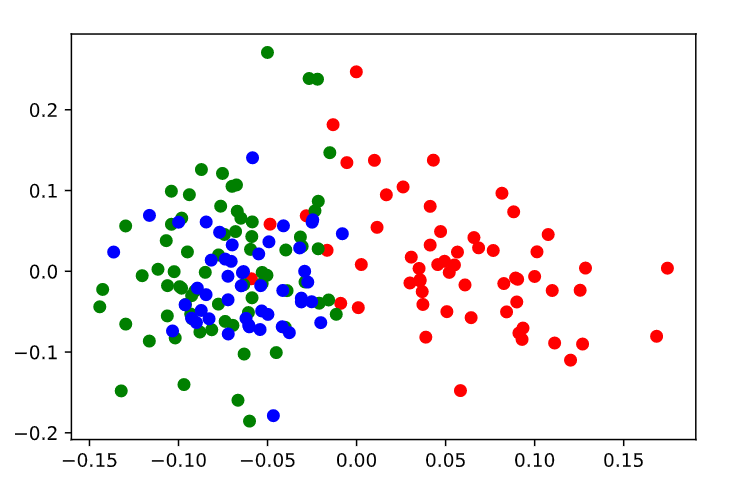
\includegraphics[width=4in]{13.png}
            \end{center}
\end{itemize}
\end{document}